\newcommand{\sist}[2]{\[ \left\{\begin{array}{rcl} x' &=& #1 \\ y' &=& #2 \end{array}\right. \]}

\section{Sistemas autónomos. Plano de fases}

Ya hemos pasado por un tema de sistemas lineales donde aprendimos a resolver cosas de la forma \[ \begin{cases}x'= a_{11}x + a_{12}y \\ y'=a_{21}x + a_{22}y \end{cases} \]. Ahora veremos sistemas de la forma \[ \begin{cases} x'(t) = F(x,y) \\ y'(t) = G(x,y) \end{cases} \]. Trabajaremos en dimensión dos para dibujar de forma mucho más precisa los sistemas, pero la teoría será genérica.

El detalle importante de estos sistemas es que en la parte derecha no aparece la variable $t$, lo que nos da un resultado básico: si $X(t) = (x(t), y(t))$ es solución, entonces también lo es $X_h(t) = (x(t+h), y(t+h))\; ∀h∈ℝ$. Es decir, las soluciones serán \textbf{invariantes por traslación}. Obtendremos la solución concreta al fijar el dato inicial.

En vista de este resultado, normalmente interpretaremos las soluciones $(x(t), y(t)) = σ(t)$, una curva parametrizada que dibujaremos en el plano.

Consideremos de nuevo el sistema masa resorte, con la ecuación $x'' +kx = 0$. Si lo escribimos como sistema, tenemos \[ \begin{cases} x' = y \\ x' = -kx \end{cases} \], que nos daba una solución explícita

\begin{align*}
x(t) &= A\cos \sqrt{k}t + B \sin \sqrt{k} t \\
y(t) &= B\sqrt{k}\cos \sqrt{k} t - A \sqrt{k}\sin \sqrt{k} t
\end{align*}

Supongamos que no hemos sabido resolver el sistema y no hemos encontrado la solución. Simplemente mirando el sistema deberíamos apreciar un punto importante: $x(t) = 0,\;y(t) = 0$ es una solución. Si lo pintamos en el plano de fases, la trayectoria sería un único punto en el origen. Se trata de una solución estacionaria o punto de equilibrio.

\begin{definition}\name{Punto}[de equilibrio]
En general, diremos que $(a,b)$ es un punto de equilibrio si y sólo si $F(a,b) = G(a,b) = 0$.
\end{definition}

Esto nos da un primer camino a estudiar: la \textbf{estabilidad}.

El segundo problema a estudiar sería el comprobar si hay \textbf{trayectorias cerradas}. Es decir, queremos encontrar soluciones periódicas. Encontraremos un problema similar al de la estabilidad: ¿qué pasa cuando cogemos una solución que pasa por un punto cercano a una trayectoria cerrada? ¿Sigue estando cerrada o se abre?

Volviendo al problema del sistema masa-resorte: si sabemos que buscamos una curva parametrizada, ¿podemos escribirlo como conjunto de nivel? No siempre es posible pero a veces funciona. En el caso de que efectivamente podamos eescribir la solución como conjunto de nivel $E(x,y) = C$, tendríamos que

\begin{gather*}
\pd{E}{x}  x' + \pd{E}{y}y' = 0 \\
\pd{E}{x} y + \pd{E}{y} (-kx) = 0
\end{gather*}
o, dicho de otra forma, buscamos que $\grad E \perp (y,-kx)$. En este caso, $\grad E$ sería paralelo a $(kx,y)$ y obtendríamos las trayectorias dadas por la ecuación

\[ \frac{kx^2}{2} + \frac{y^2}{2} = C 
\]
lo que, en el plano de fases nos daría algo como la imagen \ref{img:FasesMasaResorte}. Ahora bien, ese dibujo no estaría completo: nos faltaría determinar el sentido en el que recorremos las curvas, que lo obtendríamos viendo la derivada.

\begin{figure}[hbtp]
\centering
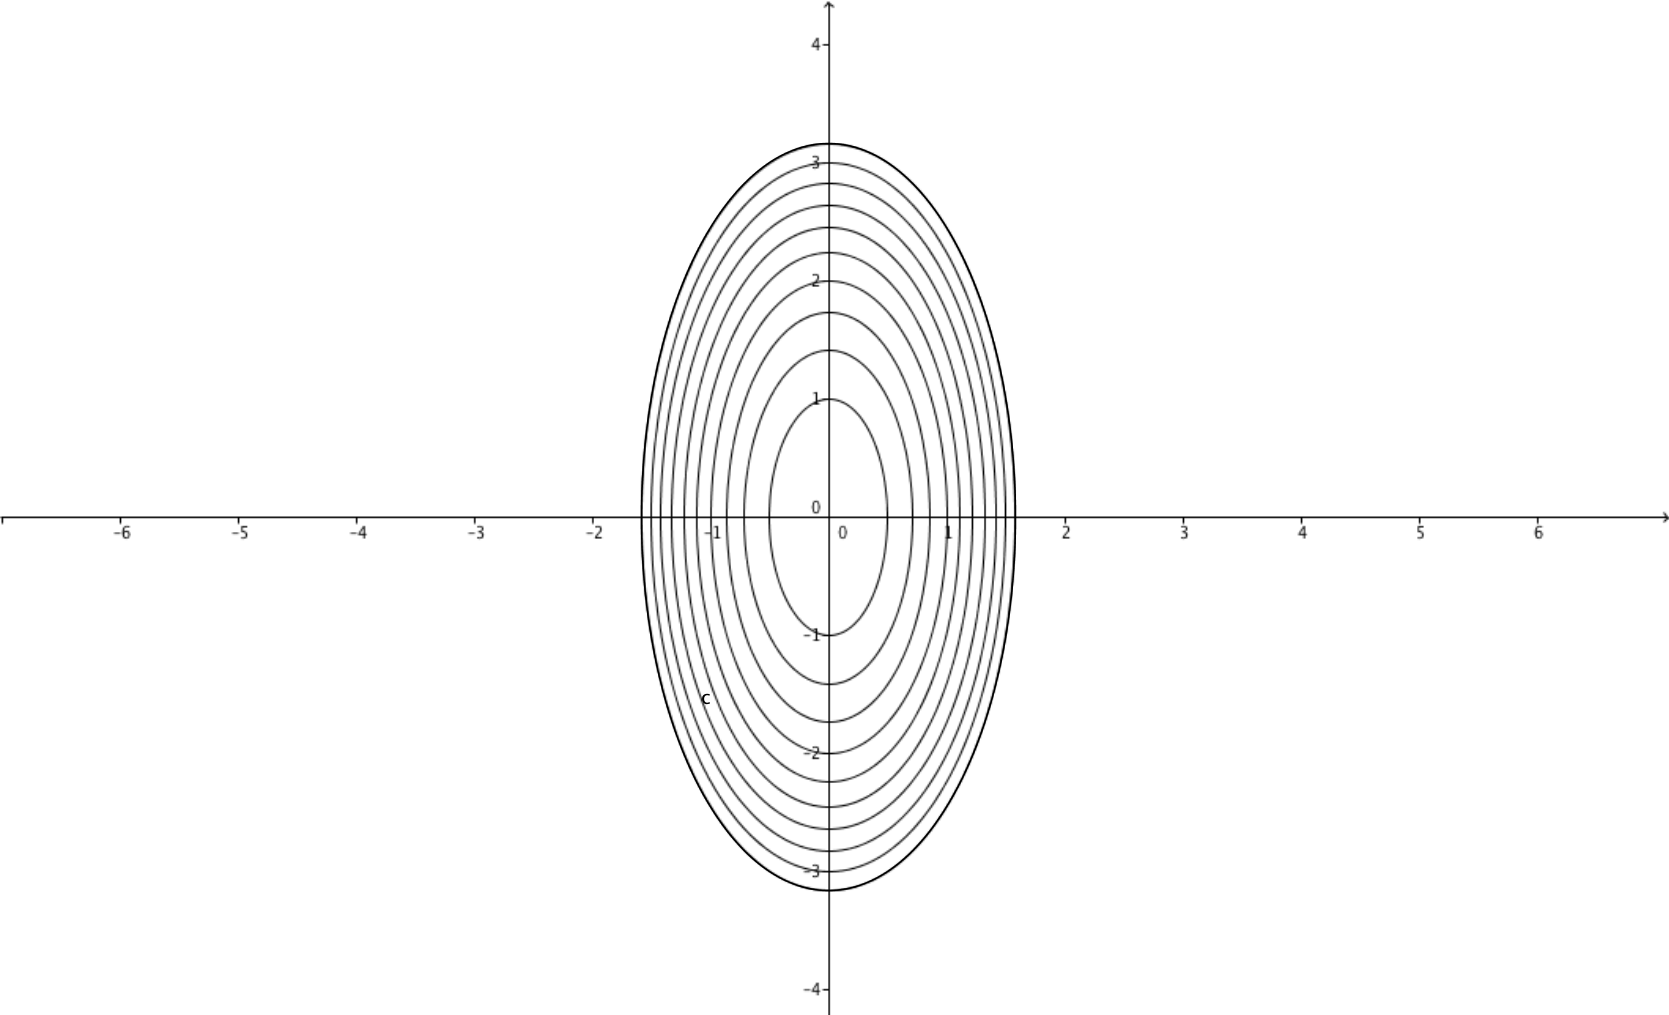
\includegraphics[width=0.8\textwidth]{img/PlanoFasesMasaResorte.png}
\caption{Plano de fases para el sistema masa-resorte}
\label{img:FasesMasaResorte}
\end{figure}

Si fuésemos físicos, veríamos que la $x$ sería la posición y $y$ la velocidad, representando en un diagrama ambas variables. Pero como no lo somos, nos la repantinfla bastante.


Si aplicamos esta misma idea a sistemas generales del estilo, \[ \begin{cases} x' = F(x,y) \\ y' = G(x,y) \end{cases} \], llegamos a la siguiente definición:

\begin{definition}\name{Integral}[ primera] Decimos que $E(x,y) ∈ C^1$ es una \textbf{integral primera} del sistema si y sólo si dado $(x(t),y(t))$ solución, entonces $E(x(t),y(t)) = C\;∀t$.
\end{definition}

Esta integral primera no siempre existe. Pero, si por ejemplo tenemos un sistema \[ \begin{cases} x' = \pd{H}{y}(x,y) \\ y' = -\pd{H}{x}(x,y) \end{cases} \] la integral primera es inmediata: $H(x,y) = C$. Los sistemas con este tipo de estructura se llaman \textbf{sistemas hamiltonianos}\index{Sistema!hamiltoniano}.

En el caso general, si tenemos una integral primera $E(x,y) = C$, entonces

\[ 0 = \pd{E}{x}x' + \pd{E}{y} y' = \pd{E}{x}F + \pd{E}{y} G 
\]
lo que nos dice que buscamos $\grad E \perp (F,G)$ o, lo que es lo mismo, $\grad E \parallel (-G,F)$. Esto nos llevaría a que si \[ -\pd{G}{y} = \pd{F}{x}\] entonces tenemos que $(-G,F) = \grad V$ para un potencial $V$, y entonces podremos tomar $E\equiv V$. Si no encuentras esto, podemos buscar un factor integrante\footnote{Y lloras. Mucho.}.

\begin{example}
\[\begin{cases}x' = y \\ y' = 1+x^2 \end{cases} \]

Buscamos una solución de la forma $E(x(t), y(t)) = C$ que cumple

\[ \grad E \perp (y, 1+x^2) \implies \grad E (1+x^2,-y) \]

Necesitamos entonces poder escribir $(1+x^2,-y)$ como $\grad V$, el gradiente de un potencial. Para ello, tendría que cumplirse que

\[ \pd{}{y}(1+x^2) = \pd{}{x}(-y) \]

Efectivamente, en este caso se cumple y existe $V$. Integrando:

\begin{gather*}
\pd{V}{x} = 1+x^2 \implies V = x + \frac{x^3}{3} + C(y) \\
-y \stackrel{?}{=} \pd{V}{y} = C'(y) \implies C(y) = \frac{-y^2}{2}
V(x,y) = x + \frac{x^3}{3} -\frac{y^2}{2}
\end{gather*}

Por lo tanto, las soluciones serán las dadas por las curvas $V(x(t), y(t)) = C$, dibujadas en la figura \ref{imgGranos}. Sólo faltaría el sentido en el que se recorren las curvas. Viendo las derivadas, vemos que $y'>0$ y que por lo tanto se recorren hacia arriba siempre, hacia la derecha cuando $y$ es positivo y hacia la izquierda en otro caso.

\end{example}

\begin{figure}
\centering
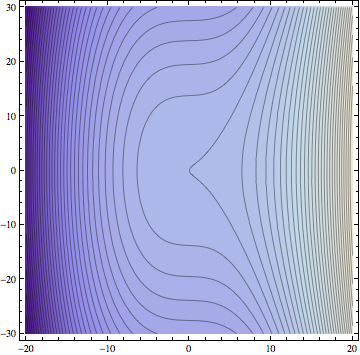
\includegraphics[width=0.5\textwidth]{img/Grano.png}
\caption{Conjuntos de nivel de la función $x + \frac{x^3}{3} -\frac{y^2}{2}$.}
\label{imgGranos}
\end{figure}

\begin{example}
\[ \begin{cases} x' = x(1+y) \\ y'=-y(1+x) \end{cases} \]

Buscamos de nuevo una posible función potencial. Hacemos las derivadas cruzadas:

\begin{gather*}
\pd{}{y} (y(1+x)) = 1+x \\
\pd{}{x} (x(1+y)) = 1+y
\end{gather*}

No existe un potencial que resuelva esta ecuación. Ahora bien, podemos buscar una función μ tal que $(μ(-G),μF)  = \grad V$. Derivamos de nuevo

\begin{align*}
\pd{}{y} (μy(1+x)) &\stackrel{?}{=} \pd{}{x} (μx(1+y)) \\
(1+x)\left(\pd{μ}{y} y + μ\right) &= (1+y)\left(\pd{μ}{x}  + μ\right)
\end{align*}

y si miramos, podremos encontrar un factor integrante.
\end{example}

\begin{example}[Tiburones en el océano]
Suponiendo que no hubiese predadores, el número de presas $x$ variaría linealmente con la tasa de supervivencia $a$, que depende de la diferencia entre mortalidad y natalidad. Es decir, \[ x' = ax \].

Con predadores, la ecuación se transformaría en \[ x' = a(y) x \], con $a$ dependiendo del número de predadores $y$. Si consideramos que $a(y)$ es una recta, por simplificar el modelo, la ecuación sería \[ x' = ax - bxy \].

Por otra parte, podemos considerar que la población de predadores crece con \[ y' = -cy + dxy \].

Transformando un poco las ecuaciones, llegamos al problema \[ \begin{cases} x' = x(a-by) \\ y' = y(-c+dx) \end{cases} \], que son las llamadas \textbf{ecuaciones de Volterra}.

Este problema tiene puntos críticos $F=G=0$. Si $F=0$, podemos tener $x=0$, el caso obvio de que no hay ni presas ni predadores. El otro es que $y=\frac{a}{b}$, que nos da que para que $G=0$ debe de ser $x=\frac{c}{d}$, lo que nos daría un punto de equilibrio.

Si añadimos al sistema a los pescadores, con influencia ε ($a\to a + ε$, $c\to c+ ε$), el punto de equilibrio pasa a ser $\displaystyle \left(\frac{a-ε}{b}, \frac{c+ε}{d}\right)$, un punto más abajo y a la derecha. Es decir, se favorece la aparición de presas y la disminución de la proporción de predadores. En la segunda guerra mundial, al bajar la pesca el movimiento se invirtió y aumentó el porcentaje de tiburones.

Ahora bien, la naturaleza no siempre se mantiene en el punto de equilibrio, sino que hay oscilaciones. Veámoslo resolviendo el sistema. Buscamos una función $E(x,y) = C$. Las derivadas cruzadas no son iguales, por lo que hay que buscar un factor integrante $μ(x,y)$ tal que

\[ \pd{}{y}(μ(x,y)(cy -dxy)) = \pd{}{x} (μ(x,y) (ax-bxy)) \]

Haciendo la cuenta, sale $μ(x,y) = \frac{1}{xy}$. La solución es entonces

\[ \grad V = \left(\frac{1}{xy}(xy-dxy),\frac{1}{xy}(ax-bxy)\right)= \left(\frac{c}{x}-d,\frac{a}{y}-b\right) 
\]
de donde podemos sacar \[ V(x,y) = a \log y - b y + c \log x - d x \].

Sólo nos interesa lo que pasa en el primer cuadrante (posiciones negativas no nos gustan). Lo que obtenemos son trayectorias cerradas alrededor de un punto de equilibrio (figura \ref{imgPoblaciones})
\end{example}

\begin{figure}[hbtp]
\centering
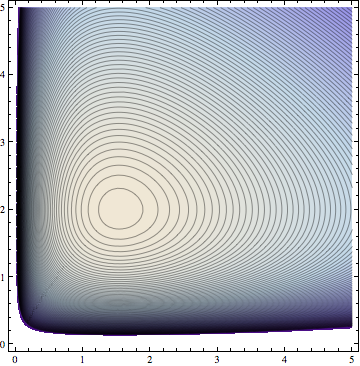
\includegraphics[width=0.5\textwidth]{img/Poblaciones.png}
\caption{Evolución de presas y depredadores.}
\label{imgPoblaciones}
\end{figure}

\begin{theorem}
Sea $(x_1(t), y_1(t))$ una solución tal que $(x_1(t),y_1(t)) ∈ γ\; ∀t$ donde γ es una curva en el plano de fases.

Sea $(x_2(t), y_2(t))$ otra solución y supongamos que existen $t_1, t_2 ∈ ℝ$ tales que  $(x_1(t_1), y_1(t_1)) = (x_2(t_2),x_2(t_2))$. Entonces $(x_2(t), y_2(t)) ⊆ γ$.

Dicho de otra forma, si dos curvas solución se cortan entonces son la misma.
\end{theorem}

\begin{proof}
Sean $(x_h(t),y_h(t)) = (x_1(t+h), y_1(t+h))$. Sabemos que si $(x_1,y_1)$ es solución y estamos en un sistema autónomo, entonces $(x_h, y_h)$ también es solución. En particular, para $h=t_1 - t_2$ tenemos que \[ (x_{t_2 - t_1}(t),y_{t_2 - t_1}(t)) = (x_1(t+t_1-t_2),y_1(t+t_1-t_2)) \].

En el punto $t=t_2$, nos queda \[ (x_{t_2 - t_1}(t_2),y_{t_2 - t_1}(t_2)) = (x_1(t_1),y_1(t_1)) \].

Tenemos dos soluciones del sistema que en el instante inicial pasan por el mismo punto. Aplicando el teorema de existencia y unicidad, tenemos que $(x_{t_2 - t_1},y_{t_2 - t_1})\equiv (x_2,y_2)$, que no es más que una traslación de la solución original $(x_1,y_1)$.
\end{proof}

\subsection{Clasificación de puntos críticos}

Partimos del sistema \[ \begin{cases} x' = ax + by \\ y' = cx + dy \end{cases} \] con $a,b,c,d∈ℝ$, que viene de una \textit{linealización} por Taylor de cualquier sistema.

¿Cuántos puntos críticos tenemos? Sabemos que siempre tenemos al menos el $(0,0)$ como punto crítico. Si además la matriz $\begin{pmatrix} a & b \\ c & d \end{pmatrix}$ tiene determinante cero, tendremos una recta de puntos críticos.

Para el análisis, empezaremos suponiendo que $(0,0)$ es un punto crítico aislado, es decir, con \[ \det \begin{pmatrix} a & b \\ c & d \end{pmatrix} ≠ 0 \].

Vamos a ir paso a paso distinguiendo los distintos casos que nos podemos encontrar al resolver este sistema.

\subsubsection{Sistemas con autovalores reales}

\paragraph{Caso 1.1: $0< λ_1 < λ_2$}. Con esta información, la solución general es

\[ \begin{pmatrix} x(t) \\ y(t) \end{pmatrix} = A e^{λ_1t}\begin{pmatrix} u_1 \\ u_2\end{pmatrix} + B e^{λ_2t} \begin{pmatrix} v_1 \\ v_2 \end{pmatrix} \].

En esta ecuación está toda la información que tenemos que tener sobre el plano de fases. Tenemos varias opciones.

Si $A = 0$, la solución es \[ B e^{λ_2t} \begin{pmatrix} v_1 \\ v_2 \end{pmatrix} \]. Es decir, que si $B>0$ tendremos una semirrecta en la dirección de $\vv$, y si es negativo una semirrecta en la dirección contraria. La solución sería análoga para $B=0$. Podemos ver en la figura \ref{imgABUnoCero} el esquema de las soluciones.

\begin{figure}[hbtp]
\inputtikz{8-ABUnoCero}
\caption{Posibles soluciones para $A=0$ ó $B=0$.}
\label{imgABUnoCero}
\end{figure}

¿Qué ocurre cuando ni $A$ ni $B$ son cero? La solución general es \[ \begin{pmatrix} x(t) \\ y(t) \end{pmatrix} = A e^{λ_1t}\vu + B e^{λ_2t} \vv \]. Podemos sacar factor común $e^{λ_1t}$ para tener

\[ \begin{pmatrix} x(t) \\ y(t) \end{pmatrix} = e^{λ_1t} \left(A\vu + Be^{(λ_2-λ_1)t} \vv\right) \].

Es decir, que cuando $t\to -∞$, $Be^{(λ_2-λ_1)t} \to 0$ y por lo tanto la trayectoria será tangente al vector $\vu$. Si lo que hacemos es sacar factor común $e^{λ_2}$, tenemos

\[ \begin{pmatrix} x(t) \\ y(t) \end{pmatrix} = e^{λ_2t} \left( Ae^{(λ_1-λ_2)t}\vu + B \vv\right) \].

Así, cualquier trayectoria en este caso acabará siendo paralela al vector $\vv$. Las trayectorias salen del origen tangentes a $\vu$ y cuando $t$ crece tienden a ser paralelas a $\vv$. Este último vector es la dirección principal, ya que atrae a todas las trayectorias salvo a la recta $\vu$ (cuando $A=0$).

\begin{figure}[hbtp]
\inputtikz{8-ABNoCero}
\caption{Posibles soluciones (en azul) para $A=0$ ó $B=0$ con ambos autovalores positivos.}
\label{imgABNoCero}
\end{figure}

\paragraph{Caso 1.2: $λ_1 < 0 < λ_2$}. La solución es la misma que antes, \[ \begin{pmatrix} x(t) \\ y(t) \end{pmatrix} = A e^{λ_1t}\vu + B e^{λ_2t} \vv \].

Cuando $A=0$, tenemos el mismo caso de antes. Ahora bien, cuando $B=0$, al ser el autovalor negativo las soluciones \textit{vienen} de infinito. Es decir, tenemos el caso de la figura \ref{imgAB_AVN_UnoCero}

\begin{figure}[hbtp]
\inputtikz{8-AB_AVN_UnoCero}
\caption{Las dos posibles rectas solución para un sistema autónomo con un autovalor negativo y otro positivo, con $A=0$ ó $B=0$.}
\label{imgAB_AVN_UnoCero}
\end{figure}

Cuando $A,B≠0$, siguiendo el mismo procedimiento de factores comunes de antes, tenemos que tanto en $+∞$ como en $-∞$ explotan. Cuando $t\to -∞$, estamos \textit{lejos} y paralelos a $\vu$. Cuando $t\to + ∞$, la trayectoria también se irá lejos en la dirección de $\vv$, tal y como refleja la figura \ref{imgAB_AVN_NoCero}.

\begin{figure}[hbtp]
\centering
\inputtikz{8-AB_AVN_NoCero}
\caption{En azul, posibles soluciones de un sistema autónomo con un autovalor negativo y otro positivo, con $A≠0,B≠0$.}
\label{imgAB_AVN_NoCero}
\end{figure}

\paragraph{Caso 1.3 $λ_1<λ_2<0$}

\footnote{A completar}

\paragraph{Caso 1.4 $λ_1=λ_2 > 0$}

Si tenemos λ autovalor doble, tenemos dos opciones. O bien hay dos vectores independientes $\vv,\vu$, y entonces podremos escribir la solución general
\[ \begin{pmatrix} x(t) \\ y(t) \end{pmatrix} = e^{λt}\left(A\vu + B\vv\right) \].

Las soluciones serán por lo tanto semirrectas que salen con cualquier dirección (la que diga $\left(A\vu + B\vv\right))$), tal y como aparece en la figura \ref{imgAB_AVDob_VI}.

\begin{figure}[hbtp]
\inputtikz{8-AB_AVDob_VI}
\caption{En azul, posibles soluciones de un sistema autónomo con un autovalor negativo y otro positivo, con $A≠0,B≠0$.}
\label{imgAB_AVDob_VI}
\end{figure}

Si tenemos un sólo autovector independiente, necesitamos otro vector. Buscamos la matriz fundamental Φ:

\[ Φ = \begin{pmatrix}
u_1 & w_1 \\ u_2 & w_2
\end{pmatrix} \exp \left[\begin{pmatrix}
λ & 1 \\ 0 & 1
\end{pmatrix} t \right] = \begin{pmatrix}
e^{λt} u_1 & te^{λt} u_1 + e^{λt} w_1 \\
e^{λt} u_2 & te^{λt} u_2 + e^{λt} w_2
\end{pmatrix} \]
y por lo tanto la solución general es

\[ \begin{pmatrix}
x(t) & y(t)
\end{pmatrix} = Ae^{λt} \vu + B (te^{λt} \vu + e^{λt}\vv) \].

Si sacamos factor común, veríamos que cuando $t\to -∞$, la solución parte del origen y \textit{explota} cuando $t\to +∞$. Es decir, algo como en la imagen \ref{imgAB_AVDob_NoVI}.

\begin{figure}[hbtp]
\inputtikz{8-AB_AVDob_NoVI}
\caption{En azul, posibles soluciones de un sistema autónomo con autovalor doble y un único autovector independiente. En verde la recta que pasa por todos los puntos con $x'=0$.}
\label{imgAB_AVDob_NoVI}
\end{figure}

Estaríamos entonces ante un \textbf{nodo impropio inestable}.

\paragraph{Caso 1.5: $λ_1 = λ_2 < 0$} En este caso estamos ante la misma situación que antes, sólo que cambiando la estabilidad. Las soluciones irán \textit{hacia}. Tendremos un \textbf{nodo impropio asintóticamente estable}.

\subsubsection{Sistemas con autovalores complejos}

Supongamos que tenemos un autovalor $λ_1 = α+ β\imath$ con autovector asociado $\begin{pmatrix}
u_1 + \imath v_1 \\ u_2  + \imath v_2
\end{pmatrix}$. Con esta información, $λ_2$ será el conjugado y el autovector será el conjugado igualmente. La ventaja es que teniendo autovalores complejos nos ahorramos el caso de que puedan repetirse.

Una solución particular es

\[ \vz_1(t) = e^{αt} (\cos β t + \imath \sin βt ) \begin{pmatrix}
u_1 + \imath v_1 \\ u_2 + \imath v_2
\end{pmatrix} \]

y la otra sería $\vz_2(t)$, el conjugado de $\vz_1(t)$ que no voy a volver a copiar. La combinación lineal de ambas será la solución general. Queremos las soluciones reales, así que sacamos la parte real e imaginaria (ambas operaciones son combinaciones lineales):

\begin{gather*}
\Re z_1 = \frac{z_1+z_2}{2} = e^{at} \underbrace{\begin{pmatrix}
u_1\cos βt - v_1 \sin β t \\
u_2\cos βt - v_2 \sin β t
\end{pmatrix}}_{J} \\
\Im z_1 = \frac{z_1-z_2}{2\imath} = e^{αt} \underbrace{\begin{pmatrix}
v_1\cos βt + u_1 \sin β t \\
v_2\cos βt + u_2 \sin β t
\end{pmatrix}}_{K} \end{gather*}

Entonces tenemos una solución general real

\[ \begin{pmatrix}
x(t) \\ y(t)
\end{pmatrix} = e^{αt} \left(A J + B K \right) \]


\paragraph{Caso 2.1: $α=0$} Tanto en $J$ como $K$ tenemos senos y cosenos. Al ser una expresión periódica, las trayectorias son curvas cerradas, más concretamente elipses (ver figura \ref{imgSA-Elipses})

\begin{figure}[hbtp]
\inputtikz{8-SA_Elipses}
\caption{Las soluciones son elipses centradas alrededor del origen.}
\label{imgSA-Elipses}
\end{figure}

Para completar el dibujo, necesitaremos el sentido de las elipses, los puntos de tangente vertical ($ax+by=0$) y los de tangente horizontal (los que cumplen $cx+dy = 0$).

¿Qué tipo de estabilidad tenemos en este caso? No es asintóticamente estable (no tendemos al origen) pero si nos alejamos un poco nos quedamos cerca. El punto se llamará \textbf{centro estable}.\index{Centro!estable}

\paragraph{Caso 2.2: $α>0$} En este caso, tendremos espirales que se alejan del origen según crece $t$. El punto es un \textbf{ inestable}.\index{Foco!inestable}

\begin{figure}[hbtp]
\inputtikz{8-SA_Espirales}
\caption{Distintas espirales solución según sea $α>0$ (izquierda) o $α>0$ (derecha).}
\label{imgSAEspirales}
\end{figure}

\paragraph{Caso 2.3: $α<0$} Análogamente, las espirales aquí se acercarán al origen. El punto es un \textbf{foco estable}\index{Foco!estable}.

En ambos casos tenemos que identificar el sentido de giro, puntos de tangencia vertical y puntos de tangencia horizontal.

Veamos algunos ejemplos:

\begin{example}
Sea el sistema siguiente
\begin{equation*}
\left\lbrace
\begin{array}{l}
	x' = 4x+2y\\
	y'=x+2y
\end{array}
\right.
\end{equation*}

Este sistema da lugar a la matriz $\begin{pmatrix}
4& 2\\1& 2
\end{pmatrix}$
cuyo determinante es distinto de cero, de lo que deducimos que $(0,0)$ es el \textbf{único punto crítico.}

Pasamos a calcular los autovalores y autovectores:

$$0 = \begin{vmatrix}
4-\lambda& 2\\1& 2-\lambda
\end{vmatrix} = (4-\lambda)(2-\lambda)-2 = \lambda^2-6\lambda+6$$

Los autovalores son por tanto
$$\lambda = \frac{6\pm \sqrt{36-24}}{2} = 3\pm \sqrt{3}$$
Como los autovalores son distintos y positivos tenemos un \textbf{nodo inestable.}

Pasamos a calcular los autovectores:
$$\begin{pmatrix}
4& 2\\1& 2
\end{pmatrix}\begin{pmatrix}
u_1\\ u_2
\end{pmatrix}=(3+\sqrt{3})\begin{pmatrix}
u_1\\ u_2
\end{pmatrix}$$
De donde obtenemos el sistema
\begin{equation*}
\left\lbrace
\begin{array}{l}
	4u_1+2u_2=(3+\sqrt{3})u_1\\
	u_1+2u_2 = (3+\sqrt{3})u_2
\end{array}
\right.
\end{equation*}

de donde sacamos que $\vec{u} = \begin{pmatrix}
1\\\frac{-1+\sqrt{3}}{2}
\end{pmatrix}$

De la misma forma calculamos $\vec{v} = \begin{pmatrix}
1\\\frac{-1-\sqrt{3}}{2}
\end{pmatrix}$

A partir de aquí podemos dibujar el plano de fases.

Tenemos la solución general

$$\begin{pmatrix}
x(t)\\y(t)
\end{pmatrix} = Ae^{(3+\sqrt{3})t}\begin{pmatrix}
1\\\frac{-1+\sqrt{3}}{2}
\end{pmatrix}+Be^{(3-\sqrt{3})t}\begin{pmatrix}
1\\\frac{-1-\sqrt{3}}{2}
\end{pmatrix} = $$

$$e^{(3+\sqrt{3})t}\{ A\vec{u} + Be^{(-2\sqrt{3})t}\vec{v} \} = e^{(3-\sqrt{3})t}\{ Ae^{(2\sqrt{3})t}\vec{u} +B\vec{v} \}$$

\textbf{dibujito}
\end{example}

\begin{example}
Sea el sistema siguiente
\begin{equation*}
\left\lbrace
\begin{array}{l}
	x' = 4y\\
	y'= -x+4y
\end{array}
\right.
\end{equation*}


Calculamos los autovalores
$$0 = \begin{vmatrix}
-\lambda & 4\\ -1& 4-\lambda
\end{vmatrix} = \lambda^2-4\lambda+4$$
$$\lambda = \frac{4\pm \sqrt{16-16}}{2} = 2\text{ (doble)}$$

Como los autovalores son positivos tenemos un nodo impropio inestable.

Pasamos a calcular los autovectores.
Tenemos
$$\begin{pmatrix}
0& 4\\-1& 4
\end{pmatrix}\begin{pmatrix}
u_1\\u_2
\end{pmatrix} = 2\begin{pmatrix}
u_1\\u_2
\end{pmatrix}$$
que da lugar al sistema:

\begin{equation*}
\left\lbrace
\begin{array}{l}
	4u_2 = 2u_1\\
	-u_1+4u_2 = 2u_2
\end{array}
\right.
\end{equation*}
de donde sale que $\vec{u}= \begin{pmatrix}
2\\1
\end{pmatrix}$

Vemos que \textbf{no} hay un segundo autovector independiente, por tanto la solución general vendrá dada a partir de la forma canónica de Jordan.

Hay que calcular los puntos de tangente vertical y horizontal para comprobar el sentido de las soluciones en el plano de fases.

A partir del sistema, sabemos que
\paragraph{Tangente (0, *)}
\begin{equation*}
\left\lbrace
\begin{array}{l}
	x^\prime = 0 \iff y=0\\
	y^\prime = -x+4y
\end{array}
\right.
\end{equation*}

De ambas ecuaciones tenemos que $y^\prime = -x$

\paragraph{Tangente (*, 0)}
No me ha dado tiempo porque se pone en medio y no veo.

\textbf{dibujito}

\end{example}

Resumamos lo visto hasta ahora
\paragraph{Autovalores reales}
\begin{itemize}
\item $0< \lambda_1 < \lambda_2 \rightarrow$ Nodo inestable.
\item $\lambda_1 < 0 < \lambda_2 \rightarrow$ Silla (inestable).
\item $\lambda_1 < \lambda_2 < 0 \rightarrow$ Nodo asintóticamente estable.
\item $\lambda_1 = \lambda_2 > 0 \rightarrow$ Nodo impropio inestable.
\item $\lambda_1 = \lambda_2 < 0 \rightarrow$ Nodo impropio asintóticamente estable.
\end{itemize}

\paragraph{Autovalores complejos}
Geométricamente, los autovalores complejos implican un giro, donde la parte real indica si la gráfica se abre o se cierra.
Si los autovalores son de la forma
$$\lambda = \alpha \pm i\beta$$
\begin{itemize}
\item $\alpha > 0 \rightarrow$ Foco (espiral) inestable.
\item $\alpha = 0 \rightarrow$ Centro estable.
\item $\alpha < 0 \rightarrow$ Foco (espiral) asintóticamente estable.
\end{itemize}

\textbf{Observación 1}

Estabilidad $\leftrightarrow$ parte real de los autovalores $
\left\lbrace
\begin{array}{l l}
> 0 \rightarrow &\text{ inestable}\\
= 0 \rightarrow &\text{ estable}\\
< 0 \rightarrow &\text{ asintoticamenteestable}\\
\end{array}
\right.
$

\textbf{Observación 2}

Estabilidad \textbf{sensible} bajo permutaciones: $A, B, C$ son casos límite o frontera.

\textbf{Diagrama}

Hasta ahora hemos calculado los autovalores de la matriz de la siguiente forma:

$$0 = \begin{vmatrix}
a-\lambda& b\\c& d-\lambda
\end{vmatrix} = (a-\lambda)(d-\lambda)-bc = \lambda^2-\lambda(a+d)+(ad-bc) = \lambda^2-T\lambda+D$$
Donde
\begin{itemize}
\item $T = a+d$ Traza de la matrix
\item $D = ad-bc$ Determinante de la matrix
\end{itemize}
Tenemos entonces que
$$\lambda = \frac{T\pm\sqrt{T^2-4D}}{2}$$
El hecho de que los valores de $\lambda$ sean complejos o no depende del radicando anterior.

(\textbf{Dibujito de una parábola $D=\frac{T^2}{2}$ donde los ejes son y=D, x=T})

Según las relaciones que haya entre el determinante de la matriz y su traza tenemos casos distintos:
\begin{itemize}
\item Si la traza es 0, estamos en el eje $D$ y tendremos un centro estable.
\item Si $D>\frac{T^2}{4}$ estamos en el primer cuadrante, por encima de la parábola y tendremos un foco inestable.
\item Si $D>\frac{T^2}{4}$ estamos en el segundo cuadrante, por encima de la parábola y tendremos un foco estable.
\item DESCRIBIR EL RESTO DE CASOS.
\item En el caso de que $D=0$ estamos en el eje $T$, que
\end{itemize}

La zona de estabilidad es justamente el segundo cuadrante.

\subsection{Método de linealización}

\begin{definition}\name[Punto]{crítico estable}\label{defPuntoEstable}

Dado un sistema \[ \begin{cases} x' = F(x,y) \\ y'= G(x,y) \end{cases} \] con $(x_0, y_0)$ punto crítico. Se dice que $(x_0, y_0)$ es un punto crítico estable si y sólo si $∀R>0 \, ∃r > 0$ tal que si $\norm{(x(t_0),y(t_0)) - (x_0,y_0)} < R$ entonces $\norm{(x(t), y(t)) -(x_0, y_0)} < r \; ∀t > t_0$.

\end{definition}

\begin{definition}\name[Punto]{asintóticamente estable}

En las mismas hipótesis de la definición anterior, decimos que $(x_0,y_0)$ es asintóticamente estable si y sólo es estable y $∃R>0$ tal que si $\norm{x(t_0), y(t_0)) - (x_0,y_0)} < R$ entonces $\lim_{t\to ∞} (x(t), y(t)) = (x_0, y_0)$.
\end{definition}

\begin{figure}[hbtp]
\inputtikz{8-PuntosEstables}
\caption{En estos dos gráficos, el origen es punto crítico estable y asintóticamente estable respectivamente.}
\end{figure}

Notamos que un punto estable no tiene por qué ser asintóticamente estable. Por ejemplo, el centro de una elipse es un punto estable pero no asintóticamente estable, ya que las trayectorias no tienden al origen.

Estas dos definiciones tienen como objetivo el \textbf{método de linealización}. Tenemos $F,G∈C^1$ con $F(x_0,y_0) = G(x_0, y_0) = 0$. Si hacemos el desarrollo de Taylor, tenemos que

\begin{gather*}
F(x,y) = F(x_0, y_0) + \pd{F}{x}(x_0,x_0) · (x-x_0) + \pd{F}{y}(x_0, y_0) · (y-y_0) + \mathrm{error}_F \,(x,y) \\
G(x,y) = G(x_0, y_0) + \pd{G}{x}(x_0,x_0) · (x-x_0) + \pd{G}{y}(x_0, y_0) · (y-y_0)+ \mathrm{error}_G \,(x,y)
\end{gather*}

Por lo tanto, cerca de $(x_0, y_0)$ tenemos

\begin{equation} \label{eqML_TaylorNoErr}
\begin{matrix}
x' &\simeq&  a(x-x_0) + b(y-y_0) \\
y' &\simeq& c(x-x_0) + d(y-y_0)
\end{matrix}
\end{equation}

Haciendo un cambio de variable para quitarnos la traslación, llegamos a

\begin{equation} \label{eqML_Trasl}
\begin{matrix}
\tilde{x}' &=& a\tilde{x} + b \tilde{y} \\
\tilde{y}' &=& c\tilde{x} + d \tilde{y}
\end{matrix}
\end{equation}


El comportamiento cerca del punto crítico $(x_0, y_0)$ para el sistema \eqref{eqML_TaylorNoErr} es el mismo que el de \eqref{eqML_Trasl}. Estudiaremos el segundo ya que es tipo de sistema que ya habíamos visto.

Supongamos que tenemos un sistema con puntos críticos $(0,0)$ y $(1,1)$. Hacemos la linealización en $(0,0)$, de tal forma que tendríamos la matriz del sistema linealizado en $(0,0)$:

\begin{equation} \label{eqML_MatSistLin} \begin{pmatrix}
\pd{F}{x}(0,0) & \pd{F}{y}(0,0) \\
\pd{G}{x}(0,0) & \pd{G}{y}(0,0)
\end{pmatrix} \end{equation}

Supongamos que esta matriz nos da autovalores $1$ y $-1$ con autovectores $(1,1)$ y $(1,-1)$. Automáticamente vemos que es un punto de silla y que las soluciones alrededor de ese punto tendrán la forma de la figura \ref{imgML_Silla}

\begin{figure}[hbtp]
\inputtikz{8-ML_Silla}
\caption{Distribución de las soluciones alrededor de los puntos críticos $(0,0)$ (izquierda) y $(1,1)$ (derecha).}
\label{imgML_Silla}
\end{figure}

\footnote{Revisar orientación de las soluciones en \ref{imgML_Silla}.}

Si linealizamos en $(1,1)$, nos saldría una matriz similar a \eqref{eqML_MatSistLin}, pero con las derivadas evaluadas en $(1,1)$. Si suponemos que tenemos autovalores $-1+\imath$ y $-1+\imath$, lo que nos daría espirales asintóticamente estables.

Tenemos las dos soluciones de la figura \ref{imgML_Silla}. ¿Cómo juntamos estas dos cosas?

\begin{figure}[hbtp]
\inputtikz{8-ML_Soluciones}
\caption{Más o menos ésta será la forma del sistema completo. Todas las soluciones a la derecha de la recta naranja caerán en las espirales que tienen como foco el $(1,1)$.}
\label{imgMLSoluciones}
\end{figure}

Si quisiésemos analizar este punto crítico, nos interesaría la recta separatriz (en naranja en la figura \ref{imgMLSoluciones}), que divide el plano en dos regiones, una en la que las soluciones se van a una espiral y otra en la que las soluciones se van a infinito.

\begin{theorem} Supongamos $(x_0, y_0)$ punto crítico, $F, G∈C^1$, con los coeficientes de Taylor de antes, y con \[ \det \begin{pmatrix}
a & b \\ c & d
\end{pmatrix} ≠ 0 \]. Trasladamos el sistema linealizado a $(0,0)$ mediante el cambio de variable $\tilde{x} = x - x_0$, $\tilde{y}= y-y_0$.

Entonces, si el punto crítico $(0,0)$ en el sistema linealizado pertenece a alguno de los casos principales (nodos propios, sillas o focos; ver imagen \ref{imgCosasRarasRualFoto}) entonces sigue siendo del mismo tipo en cuanto a forma y estabilidad en el sistema completo.

Si en el sistema linealizado tenemos un nodo impropio inestable, entonces en el sistema completo tendremos un nodo o una espiral, inestables en ambos casos.

Si tenemos un nodo impropio asintóticamente estable, en el sistema completo tendremos un nodo o espiral asintóticamente estable.

El caso peor es  si tenemos un centro estable, ya que puede ocurrir cualquier cosa.
\end{theorem}

En relación con las integrales primeras, vemos que sólo podremos expresar las soluciones como conjuntos de nivel si los puntos críticos son nodos o centros.

\begin{example}
\[\begin{cases}
x' &= x(60-3x-4y) \\
y' &= y(42-2x-3y)
\end{cases} \]

Si viésemos esto en el contexto de estudio de poblaciones, veríamos que son dos especies compitiendo por un mismo recurso limitado. Los puntos críticos son $(0,0)$, $\left(0, 14\right)$, $(20, 0)$ y $(12, 6)$. Tendremos cuatro sistemas linealizados distintos, donde tendremos que calcular autovalores y autovectores. Habrá que dibujar puntos críticos separados, discernir si estamos en los casos principales y juntarlo.

En este sistema habría que preguntar qué especie extingue a la otra. El lunes volveremos con ello.
\end{example}


Hagamos un ejemplo algo más complejo. Partimos del problema \[ \begin{cases} x' &= x(2-x-y) = F(x,y) \\ y' &= y(3-y-2x) = G(x,y) \end{cases} \] y estudiamos sus puntos críticos, que son $(0,0)$, $(0,3)$, $(2,0)$, $(1,1)$.

Aplicamos el método de linealización y obtenemos la matriz de derivadas parciales:

\[ Δ = \begin{pmatrix}
\pd{F}{x} & \pd{F}{y} \\ \pd{G}{x} & \pd{G}{y}
\end{pmatrix} = \begin{pmatrix}
2 - 2x -y & -x \\
-2y & 3-2y-2x
\end{pmatrix} \]

Vamos estudiando cada punto crítico:

\paragraph{$(0,0)$} Hallamos el valor de la matriz de derivadas parciales

\[ Δ(0,0) = \begin{pmatrix}
2 & 0 \\ 0 & 3
\end{pmatrix} \], que como ya es diagonal vemos que los autovalores son $2$ y $3$ con autovectores $\vu = (1,0)$ y $\vv=(0,1)$. Alrededor de este punto crítico, las soluciones se parecerán a la figura \ref{imgEj1_00}

\begin{figure}[hbtp]
\centering
\inputtikz{8-Ej1_00}
\label{imgEj1_00}
\end{figure}

\paragraph{$(0,3)$}. Autovalores $-3$, $-1$, autovectores correspondientes $(0,1)$, $(-1, 3)$. Las soluciones se parecen a \ref{imgEj1_03}


\begin{figure}[hbtp]
\centering
\inputtikz{8-Ej1_03}
\label{imgEj1_03}
\end{figure}

Si seguimos, llegamos a una gráfica como la de la figura \ref{imgEj1_Final}. También vemos que hay trayectorias \textbf{heteroclínicas}\index{Trayectoria!heteroclínica}, que lleva de un punto crítico a otro.

\begin{figure}[hbtp]
\centering
\inputtikz{8-Ej1_Final}
\label{imgEj1_Final}
\end{figure}

En algunos casos, no podemos aplicar la teoría directamente. En el sistema \[ \begin{cases}
x' &= y(x-2) \\ y' &= x(y-2)
\end{cases} \], lo que nos da los puntos críticos $(0,0)$ y $(2,2)$. Hallamos la matriz Δ de derivadas parciales

\[ \begin{pmatrix}
\pd{F}{x} & \pd{F}{y} \\ \pd{G}{x} & \pd{G}{y}
\end{pmatrix} = \begin{pmatrix}
y & x- 2 \\ y -2 & x \end{pmatrix} \]

En $(0,0)$ tenemos autovalores $λ=\pm 2$ con autovectores $(1,-1)$ y $(1,1)$ respectivamente, lo que nos indica que tenemos un punto de silla.

En $(2,2)$ tenemos autovalor $λ=2$ doble, con autovectores $(1,0)$ y $(0,1)$. Tenemos entonces un nodo impropio inestable y las soluciones serán rectas que parten del origen en cualquier dirección.

En el sistema completo, el primer caso se mantiene. Sin embargo, el segundo punto crítico no se mantiene. Podemos garantizar que será inestable, pero no sabemos si será un nodo inestable o si habrá un foco inestable.

Estudiamos el sistema completo para obtener alguna información adicional. Vemos que los puntos con tangente vertical son o $x=2$ ó $y=0$, y con tangente horizontal tenemos los puntos $y=2$ ó $x=2$.

A partir del estudio de este campo de pendientes, vemos que es imposible que haya una espiral en el punto $(2,2)$, ya que en algún momento tendría que tener una tangente vertical u horizontal, cosa que sabemos que no existe.

\begin{figure}[hbtp]
\inputtikz{8-Ej2}
\label{img8-Ej2}
\caption{A completar. Soluciones en el sistema completo.}
\end{figure}

También podemos ver que existen cuatro trayectorias de la forma $(x(t), 2)$ y $(2,y(t))$, es decir, las rectas marcadas en rojo y naranja en la figura \ref{img8-Ej2}

\paragraph{Vuelta al péndulo} Recordemos el sistema del péndulo simple de clases anteriores. Ahí asumíamos que las oscilaciones $x$ eran pequeñas y por lo tanto podíamos decir que $\sin x \simeq x$. Ahora vamos a olvidar esa parte y vamos a estudiar el problema para cualquier oscilación.

Escribimos la ecuación $x'' + k\sin x = 0$ en forma de sistema: \[ \begin{cases} x' &= y \\ y' &= -k \sin x \end{cases} \]. Los puntos críticos ocurren con $y=0$, $x = \pm α π$ con $α∈ℤ$. Con α par, tendremos la matriz lineal \[ \begin{pmatrix} 0 & 1 \\ -k & 0\end{pmatrix} \], y con α impar será \[ \begin{pmatrix} 0 & 1 \\ k  & 0 \end{pmatrix} \].

En el primer caso tendremos $λ=\pm \sqrt{k} \imath$ y en el segundo $λ=\pm \sqrt{k}$, lo que nos da un centro (elipses) y un punto de silla respectivamente.

Los puntos de silla se mantienen en el sistema completo, pero no los centros. Por este camino no llegamos a nada. Sin embargo, podemos aplicar el método de las \textbf{integrales primeras}.

Buscamos un potencial $E(x(t), y(t)) = C$ tal que \[ \pd{E}{x}x' + \pd{E}{y}y' = 0 \]. $(k\sin x, y)$ es un vector gradiente, así que podemos tomar \[ E(x,y) = \frac{y^2}{2} - k\cos x \].

Al trasladarlos al sistema completo, no sabíamos si los centros se convierten en focos inestables, asintóticamente estables o en centros. Pero como hemos podido escribir las curvas como conjuntos de nivel de un potencial, no hay forma de que haya espirales (focos) y por lo tanto en los puntos de la forma $(απ, 0)$ con α impar hay elipses.

\begin{figure}[hbtp]
\inputtikz{8-Pendulo}
\label{imgPendulo}
\caption{El plano de fases del péndulo, las gráficas del ángulo de oscilación en función del tiempo según la trayectoria y su \textit{traducción} al péndulo real.}
\end{figure}

En la figura \ref{imgPendulo} tendremos varias trayectorias. En naranja, la elipse, un péndulo que oscila continuamente. En rojo, el péndulo cae desde arriba y llega con velocidad 0 al mismo punto. En azul, simplemente giraría de forma continua.

Si añadiésemos el rozamiento, los puntos críticos serían focos asintóticamente estables y sillas, que se conservan en el sistema completo. Los centros pasarían a ser puntos espirales. Las trayectorias que salen de un punto de silla caerían en ese foco de la espiral.

Podemos extrapolar lo que hemos llegado con el péndulo a ecuaciones más genéricas de la forma \[ x''+f(x) = 0 \], que podemos transformar a un sistema \[ \begin{cases} x' = y \\ y' = -f(x) \end{cases} \].

Estos sistemas tienen una integral primera $E(x,y)$ tal que toda solución se puede expresar como \[ E(x(t), y(t) = C \], es decir, como los conjuntos de nivel de un potencial.

Si hacemos los cálculos, tenemos que tener $\grad E \parallel (f(x), y)$, lo que nos da \[ E(x,y) = F(x) + \frac{y^2}{2} \] donde $F' = f$. Dicho de forma física, tendríamos la conservación de la energía del sistema.

\begin{figure}[hbtp]
\inputtikz{8-EsbozoSist}
\label{imgEsbozoSist}
\caption{Esbozo de las soluciones de un sistema similar al del péndulo.}
\end{figure}

De esta ecuación podemos dar un primer esbozo del plano (figura \ref{imgEsbozoSist}). Como $x'=y$, tenemos que $x'>0$ en el semiplano superior y $x'<0$ en el semiplano inferior, además de ver que las trayectorias tienen tangente vertical en $y = 0$.

Si despejamos $y$, tenemos que $y = \pm \sqrt{2}\sqrt{C-F(x)}$, por lo que las trayectorias son simétricas con respecto al eje $x = 0$.

Esta última fórmula nos permite ver cómo son las trayectorias sabiendo sólo el dibujo de $F(x)$. Veamos cómo en otro ejemplo más, el del sistema masa resorte. En este caso teníamos \[ f(x) = \frac{k}{m}x^2;\quad F(x) = \frac{k}{2m}x^2 \equiv A x^2 \] y podemos hacer un esbozo como en la figura \ref{img8MasaResorte}.

\begin{figure}[hbtp]
\inputtikz{8-MasaResorte}
\label{img8MasaResorte}
\caption{Esbozo de las soluciones del sistema masa resorte a partir de $F(x) = A x^2$ para dos constantes $C_1$ y $C_2$}
\end{figure}

Este método nos permite estudiar sistemas en los que el método de linealización no nos serviría.

\subsection{Método directo de Liapounov}

Estudiemos este método con un ejemplo:

\[ \begin{cases} x' &= y-x(x^2+y^2) \\ y' &= -x -y(x^2+y^2) \end{cases} \]

El único punto crítico del sistema es el $(0,0)$, que aplicando el método de linealización vemos que es un centro. No podemos concluir nada sobre lo que ocurre al trasladar al sistema completo. Imaginemos que hacemos el siguiente cálculo ingenuo.

Supongamos una trayectoria $(x(t), y(t))$ y medimos el cuadrado de su distancia al origen con una función $D(t) = x^2(t) + y^2(t)$, y miramos su derivada. Si nos sale siempre positiva o siempre negativa, podremos decir que las soluciones se alejan o se acercan al punto crítico, respectivamente. En este caso,

\[ D'(t) = 2xx' + 2yy' = 2x(y-x(x^2+y^2)) + 2y(-x-y(x^2+y^2)) = -2(x^2+y^2)^2 \]

Como siempre es negativo, tenemos un punto crítico estable. Liapounov dio un paso más: ¿qué valor tiene el hecho de que hayamos elegido la distancia? Nos vale con tener una función con que en el origen valga 0 y que vaya creciendo según me aleje. La idea de Liapounov es encontrar una \textit{distancia} de tal forma que su derivada sea siempre negativa o positiva.


\begin{definition}\name[Función]{de Liapounov} Supongamos que tenemos un sistema \begin{equation} \begin{cases} x' = F(x,y) \\ y' = G(x,y) \end{cases} \label{eqSisLiap} \end{equation} con $(0,0)$ punto crítico aislado, y trayectorias $(x(t), y(t))$.

Una función $E(x, y)$ es una función de Liapounov para ese sistema si y sólo si

\begin{itemize}
\item $E$ es $C^1$ en algún abierto alrededor de $(0,0)$.
\item $E(x,y) > 0$ si $(x,y) ≠ 0$ y $E(0,0) = 0$.
\item $\pd{E}{x} F + \pd{E}{y} G ≤ 0 $.
\end{itemize}
\end{definition}

\begin{theorem} Si existe alguna función de Liapounov para el sistema \ref{eqSisLiap}, entonces el punto crítico $(0,0)$ es \textbf{estable}.

Si además se tiene \[ \pd{E}{x} F + \pd{E}{y} G < 0 \quad ∀(x,y) ≠ (0,0) \], además $(0,0)$ es \textbf{asintóticamente estable}. En este caso, diremos que tenemos una \textbf{función de Liapounov estricta}.
\end{theorem}

Si dibujamos la gráfica de la función de Liapounov $z=E(x,y)$, veríamos que cuando $z'(t) > 0$ la función crece por la superficie, y si es menor que cero se acercaría al origen. Nos interesa ver por lo tanto la trayectoria $(x(t), y(t))$ en la superficie dada por esa función.

Una vez que tenemos una idea del problema, vamos a demostrarlo

\begin{proof} Empezamos viendo que \[ z'(t) = \pd{E}{x}x' + \pd{E}{y}y' = \pd{E}{x} F + \pd{F}{y} \]

\paragraph{Proposición 1: Estabilidad} Queremos demostrar que $∀ R > 0,\, ∃r>0$ tal que si $\norm{(x(t_0), y(t_0))} < r$, entonces $\norm{(x(t), y(t))} < R ∀ t > t_0$ (ver la definición de punto estable en \ref{defPuntoEstable}).

Dado $R$ consideramos el conjunto ξ y su mínimo: \[ ξ = \{ E(x,y) \st \norm{(x,y)} = R\};\; m = \min ξ \]

Si $E(x(t), y(t)) < m \, ∀t$, entonces la trayectoria no corta la circunferencia.

Sabemos que $E(0,0) = 0$ y que $E$ es continua. Por lo tanto podemos tomar un $r >0$ tal que $E(x,y) < \frac{m}{2}$ si $\norm{(x,y) ≤ r}$ por continuidad.

Supongamos que en un instante $t_0$ tenemos $\norm{(x(t_0), y(t_0))} < r$. Si además sabemos que $z'(t) ≤ 0$ por ser condición de Liapounov y tenemos que $z(t_0) < \frac{m}{2}$ por el apartado anterior, tenemos que $z(t) < \frac{m}{2}\, ∀t>t_0$.

\paragraph{Proposición 2: Estabilidad asintótica} Vamos a ver cómo la condición de Liapounov estricta nos da estabilidad asintótica. Supongamos \[ \pd{E}{x}F + \pd{E}{y}G < 0 \]

Si esto es así, entonces $z'(t) < 0$. Sabemos además que $z(t) ≥ 0$. Si tenemos una función decreciente y acotada inferiormente, entonces \[ ∃\lim_{t\to∞} z(t) = L ≥ 0 \]

\begin{wrapfigure}{r}{0.4\textwidth}
\inputtikz{8-DemLiapounov}
\label{img8-DemLiapounov}
\caption{La trayectoria está confinada en la zona verde}
\end{wrapfigure}

Si $L=0$, hemos terminado. ¿Qué pasa si $L>0$, es decir, que las trayectorias se parasen antes del origen? Demostremos que esto no puede ocurrir.

Supongamos $L>0$. Nuevamente por continuidad, puedo encontrar $δ>0$ tal que $E(x,y) > \frac{L}{2}$ si $\norm{(x,y)} < δ$. En la figura \ref{img8-DemLiapounov} las trayectorias se encontrarían sólo en la zona verde. Es decir, $(x(t),y(t)) ⊆ B_R - B_δ$.

Consideramos $z'(t)$ en el compacto $B_R - B_δ$ y $-k = \max z'(t)$ en ese conjunto. Aquí tenemos que

\[ z(t) = z(t_0) + \int_{t_0}^t z'(s)\dif s ≤ z(t_0) + \int_{t_0}^t (-k)\dif s = z(t_0) - k(t-t_0) \convs[][t] - ∞ \], una contradicción dado que decíamos que $z≥0$. Por lo tanto, no puede darse el caso de que el límite sea $L>0$.
\end{proof}

Por lo tanto, con encontrar la función de Liapounov demostraríamos la estabilidad. No tenemos garantizado el encontrar esta función siempre. En sistemas físicos podemos usar la energía del sistema. También tenemos otro tipo de estrategias que veremos en varios ejemplos.

\begin{example} \[ \begin{cases} x' &= y-3x^3 \\ y' &= -x - 7y^3 \end{cases} \]

El punto crítico es $(0,0)$, y el método de linealización nos lleva a un centro. Nos deja colgados, así que buscamos una función de Liapounov $E(x,y)$ que tenga un mínimo en $(0,0)$. Una buena idea es buscar un polinomio en potencias pares de $x$ e $y$:

\[ E(x,y) = Ax^{2n} + y^{2m} \]

Ajustaremos los tres parámetros $A>0$, $n$, $m$ tales que \[ \pd{E}{x} F + \pd{E}{y} ≤ 0 \]. No tenemos garantía de encontrarla y esto no funciona siempre, pero vamos a intentarlo. Operamos

\begin{align*}
\pd{E}{x} &= 2nAx^{2n-1} \\
\pd{E}{y} &= 2my^{2m-1} \\
\pd{E}{x} F + \pd{E}{y} G &= 2nAx^{2n-1}(y-3x^3) + 2my^{2m-1}(x+7y^3) = \\
 & =2nAx^{2n-1} y - 6nAx^{2n+2} - 2my^{2m-1} x - 14my^{2m+2}
\end{align*}

En esos cuatro sumandos de ahí, hay algunos que son bien y otros que son caca. El primero y el tercero son caca porque a veces son positivos y a veces negativos. Los otros dos sí los tenemos perfectamente controlados.

En este caso, lo que haremos será cancelarlos, lo que nos da el sistema \[ \begin{cases} 2nA &= 2m \\ 2n -1 &= 1 \\  2m - 1 &= 1\end{cases} \implies n = m = A = 1 \]

La función de Liapounov sería la distancia habitual al cuadrado $E(x,y) = x^2 + y^2$ y $\pd{E}{x} G + \pd{E}{y} G = -6x^4 - 14y^4 < 0$, es decir, un punto asintóticamente estable.
\end{example}

Una de las principales ventajas del método de Liapounov es que, a diferencia del método de linealización, también vale para puntos críticos no aislados (por ejemplo, puntos críticos distribuidos en una curva que cumple $F=G=0$). El matiz es que en un punto crítico no aislado no podemos tener estabilidad asintótica.

\begin{example} \[\begin{cases} x' = -xy^4 \\ y'=yx^4 \end{cases} \]

En este caso el método de linealización no nos da puntos críticos aislados (la matriz es nula) así que vamos a Liapounov.

\begin{align*}
E(x,y) &= Ax^{2n} + y^{2m} \\
\pd{E}{x} &= 2n Ax^{2n-1} \\
\pd{E}{y} &= 2my^{2m-1} \\
\pd{E}{x}F + \pd{E}{y}G &= -2nAx^{2n}y^4 + 2my^{2m}x^4
\end{align*}

Con $2n=2m=4$ y $A<1$ tendríamos una función de Liapounov estricta. Entonces tendríamos que \[ \pd{E}{x}(-xy^4) + \pd{E}{y}(yx^4) = 4(A-1)x^4y^4 \], que es siempre menor o igual que cero. Demostramos estabilidad pero no estabilidad asintótica.

\begin{wrapfigure}{r}{0.4\textwidth}
\inputtikz{8-Ej3}
\label{img8-Ej3}
\caption{Ocho soluciones: los cuatro puntos críticos (verde) y las cuatro trayectorias (rojo).}
\end{wrapfigure}

La pregunta es si realmente no hay estabilidad asintótica o es que no hemos visto bien la función de Liapounov.

Si nos fijamos, vemos que $(0,0)$ no es un punto crítico aislado: las rectas $(x,0)$ y $(y,0)$ son también puntos críticos, y por lo tanto no podemos tener un punto asintóticamente estable.

Haciendo más cálculos, vemos que las soluciones son conjuntos de nivel de la forma \[ x^4 + y^4 = k \], como podemos ver en la figura \ref{img8-Ej3}.
\end{example}


\paragraph{Aplicación del teorema} Vamos a aplicar el teorema de Liapounov para demostrar algo que teníamos pendiente: que la estabilidad asintótica en el sistema linealizado implica estabilidad asintótica en el sistema completo.

\begin{proof}
Partimos de la siguiente notación: $(0,0)$ es un punto crítico aislado. La derivada de $x$ es

\[ x' = F(x,y) = \pd{F}{x}(0,0)x + \pd{F}{y}(0,0)y + f(x,y) \equiv ax + by + f(x,y) \].

La segunda forma equivalente parte del desarrollo de Taylor, con $f$ el error (esto es, $\lim_{(x,y)\to (0,0)} \frac{f(x,y)}{\sqrt{x^2+y^2}}$). Análogamente,

\[ y' = G(x,y) = \pd{G}{x}(0,0)x + \pd{G}{y}(0,0)y + f(x,y) \equiv cx + dy + g(x,y) \].

Recordamos ahora el diagrama de la estabilidad\footnote{Poner el diagrama} en función de la traza $T=a+d$ y del determinante $D=ad-bc$. Si tenemos estabilidad asintótica en el sistema linealizado, tenemos que $T < 0$ y que $D > 0$.

La idea de la demostración es llevar a cabo dos pasos. El primero es construir una función de Liapounov para el sistema linealizado. El segundo, comprobar que sigue siendo válida para el sistema completo en un entorno de $(0,0)$.

La función que buscaremos será de la forma \[ E(x,y) = \frac{1}{2}\left(Ax^2 + 2Bxy + Cy^2\right) \]. Sacamos factor común $A$ y completamos cuadrados:

\begin{align*}
 E(x,y) &= \frac{A}{2}\left(x^2 + 2\frac{B}{A}xy + \frac{C}{A}y^2\right) = \\
 &= \frac{A}{2}\left[\left(x+\frac{B}{A}y\right)^2 + \left(\frac{C}{A} - \frac{B^2}{A^2}\right)y^2\right]
\end{align*}

De aquí sacamos que $A>0$ y que $\frac{C}{A}>\frac{B^2}{A^2}$. Miramos ahora las derivadas parciales: queremos comprobar que $\pd{E}{x}(ax+by) + \pd{E}{y} (cx+dy) < 0$. Operando

\begin{align*}
\pd{E}{x} &= Ax+By \\
\pd{E}{y} &= Bx + Cy \\
\pd{E}{x} (ax+by) + \pd{E}{x}(cx+dy) &=
	\underbrace{(Aa+Bc)}_{-1}x^2 +
	\underbrace{(Bb+Cd)}_{-1}y^2 +
	\underbrace{(Ab+aB+Bd+Cc)}_{0}xy
\end{align*}

Buscamos los valores de $A,B,C$ que nos dan los valores que aparecen en la ecuación. Es decir, buscamos resolver el sistema

\[ \begin{cases} Aa + Bc &= -1 \\ 
Bb+Cd &= -1 \\
Ab + aB +Bd + Cc &= 0
\end{cases} \]

Una vez fijas esas constantes, nos queda  \[ \pd{E}{x} (ax+by) + \pd{E}{x}(cx+dy) = -(x^2+y^2) \], que es menor que $0$ fuera de $(0,0)$.

Con la función de Liapounov encontrada (sabemos que existe en cualquier caso), lo aplicamos al sistema completo estudiando

\begin{equation}\label{eqLiapDem1} \pd{E}{x} (ax+by +f(x,y)) + \pd{E}{x}(cx+dy+g(x,y)) = -(x^2+y^2) + \pd{E}{x} f(x,y) + \pd{E}{y}g(x,y) \end{equation}.

Habremos terminado si demostramos que eso es menor que $0$ cuando estamos cerca del origen. Recordamos que \[ \pd{E}{x} = Ax+By \; \pd{E}{y} = Bx + Cy \] y operamos:

\[ (Ax+By)f(x,y) ≤ \underbrace{\max\{\abs{A}, \abs{B}}_M (\abs{x} + \abs{y}) · \abs{f(x,y)} \]

Sabiendo que $\abs{x} = \sqrt{x^2} ≤ \sqrt{x^2+y^2}$ (análogo con $\abs{y}$), tenemos que

\[ M(\abs{x} + \abs{y}) · \abs{f(x,y)} ≤ 2M\sqrt{x^2+y^2}\abs{f(x,y)} = 2M(x^2+y^2) \frac{\abs{f(x,y)}}{\sqrt{x^2+y^2}} \]

Sustituyendo en \eqref{eqLiapDem1}

\begin{multline*} -(x^2+y^2) + \pd{E}{x} f(x,y) + \pd{E}{y}g(x,y) ≤ -(x^2+y^2) + 2M(x^2+y^2) \frac{\abs{f(x,y)}}{\sqrt{x^2+y^2}} + 2N(x^2+y^2) \frac{\abs{g(x,y)}}{\sqrt{x^2+y^2}} \\
= (x^2+y^2)\left(-1 +
	2M \underbrace{\frac{\abs{f(x,y)}}{\sqrt{x^2+y^2}}}_{(1)} +
	2N \underbrace{\frac{\abs{g(x,y)}}{\sqrt{x^2+y^2}}}_{(2)}\right) \end{multline*}

Al ser $(1)$ y $(2)$ errores que tendían a $0$ cuando $(x,y) \to (0,0)$, con una bola suficientemente pequeña tendremos que todo eso es menor que cero y tendremos por lo tanto un punto crítico asintóticamente estable en el sistema completo.

\end{proof}

\subsubsection{Funciones de Liapounov e inestabilidad}

Podemos estudiar la inestabilidad de ciertos puntos a través de las funciones de Liapounov.

La primera idea sería \textbf{invertir el sentido de tiempo}. Reparametrizamos con $s=-t$, y entonces

\begin{align*}
\tilde{x}(s) &= x(-t) \\
\tilde{y}(s) &= y(-t) \\
\tilde{x}'(s) &= -F(\tilde{x}, \tilde{y}) \\
\tilde{y}'(s) &= -G(\tilde{x}, \tilde{y})
\end{align*}

Si tenemos una función de Liapounov $E(\tilde{x}, \tilde{y})$, con \[ \pd{E}{x} (-F) + \pd{E}{y}(-G) < 0 \], es decir, estabilidad asintótica en $(\tilde{x}, \tilde{y})$, esto querría decir que  \[ \pd{E}{\tilde{x}}F + \pd{E}{\tilde{y}}G < 0 \], es decir, inestabilidad en $(x,y)$.

Este método es muy sencillo, pero perfectamente inútil para puntos de silla. En estos puntos hay zonas en las que el origen parece que atrae las trayectorias, y otras en las que parece que las rechaza. Tendríamos que tratar de encontrar un teorema que no tenga en cuenta todo el entorno del origen, sino sólo una zona - recordemos que con que haya una trayectoria el punto crítico ya es inestable -. Otro criterio más útil es el de Chetaev.

\begin{theorem} \name[Criterio]{de Chetaev} Dado el sistema de siempre \[ \begin{cases} x' = F(x,y) \\ y' = G(x,y) \end{cases} \] con $(0,0)$ punto crítico, consideramos el disco $D_R= \{ x^2 + y^2 ≤ R^2 \}$. Sea $V∈C^1(D_R)$, y un conjunto $U = \{ (x,y) ∈ D_R \st V(x,y) > 0 \}$ (ver imagen \ref{img8-Chetaev}).

Si se dan las dos condiciones siguientes:

\begin{itemize}
\item $∀δ > 0 \; ∃(x_δ,y_δ) ∈ U \st x_δ + y_δ ≤ δ^2$. Es decir, el centro no está aislado de $U$.
\item $\displaystyle\pd{V}{x}(x,y)F(x,y) + \pd{V}{y}(x,y) G(x,y) > 0\; ∀(x,y) ∈ U$. \footnote{Esta condición también nos dice que no hay más puntos críticos en $U$.}
\end{itemize}

Entonces, tenemos inestabilidad en el punto crítico.
\end{theorem}


\begin{figure}[hbtp]
\centering
\inputtikz{8-Chetaev}
\label{img8-Chetaev}
\caption{Bola de radio $R$ $D_R$.}
\end{figure}

\begin{proof}


Consideramos la trayectoria $(x(t), y(t))$ con $(x(0), y(0)) = (x_δ, y_δ)$. Como $(x_δ, y_δ) ∈ U$, entonces con $V(x_δ, y_δ) = C_δ > 0$.

Sea $g(t) = V(x(t), y(t))$. Su derivada es

\[ g'(t) = \pd{V}{x}x' + \pd{V}{y}y' = \pd{V}{x}F + \pd{V}{y}G > 0 \] según hipótesis. Es decir, que $g$ es creciente mientras $(x(t), y(t)) ⊆ U$, por lo tanto, $g(t) ≥ g(0) = C_δ > 0$.

A partir de aquí tenemos que demostrar que para cualquier punto de partida en $U$, la trayectoria se sale de la bola $D_R$. Hagámoslo por reducción al absurdo.

Supongamos que $(x(t), y(t)) ⊆ U\; ∀t≥ 0$. Como $D_R$ es un conjunto compacto y $V$ es continua, entonces $V$ alcanza su máximo $M > 0$ en $D_R$.

Sea $A_δ = \{ (x,y) ∈ D_R \st V(x,y) ≥ C_δ \}$. Si $(x(t), y(t)) ⊆ U$ y al ser $g(t) >C_δ\, ∀t ≥ 0$, resulta que $(x(t), y(t)) ⊆ A_δ\;∀t≥0$.

Este conjunto $A_δ$ es acotado por la bola de radio $R$. También es cerrado: si escribimos $A_δ = D_R \cap V^{-1}([C_δ, ∞))$, $[C_δ, ∞)$ es abierto, $V$ continua, por lo que $V^{-1}([C_δ, ∞)$ es cerrado.

Ahora consideramos \[ γ = \min_{A_δ} \pd{V}{x} F + \pd{V}{y} G \], que es positivo. Reescribimos

\[ g(t) = g(0) + \int_0^t g'(s) \dif s = C_δ + \int_0^t \pd{V}{x}F + \pd{V}{y} G \dif s ≥ C_δ + γt \], que para $t$ suficientemente grande tendremos que es mayor que $M$: $C_δ + γt > M$.

Dado que la trayectoria no puede salir de $U$ atravesando la línea $V=0$, entonces tiene que salir por el borde de la bola. Contradicción con la hipótesis, y por lo tanto la trayectoria se sale siempre y hay inestabilidad.
\end{proof}

\begin{example}[Coordenadas polares]
Tenemos el siguiente sistema

\[ \begin{cases} x' = 3x - y - ex^{x^2+y^2} \\
y' = x+ 3y -ye^{x^2+y^2} \end{cases} \]

Veamos qué pasa si pasamos a polares. El cambio de variables es

\[ \begin{cases} x = r\cos θ \\ y = r \sin θ \end{cases}
\begin{cases} r^2 = x^2+y^2 \\ \tan θ = \frac{y}{x} \end{cases}
\begin{cases} rr' = xx' + yy' \\ r^2θ' = y'x - x' y \end{cases} \]

Ahora deberíamos operar en estas ecuaciones para que todo nos quede en términos de $r$ y θ.

\begin{align*}
 rr' &= xx' + yy' = \\
 &= \cdots = \\
 &= 3(x^2+y^2) - (x^2+y^2)e^{x^2+y^2} \\
 &= 3r^2 - r^2e^{r^2} \\
 &= r^2(3-e^{r^2})
r' = r(3-e^{r^2})
\end{align*}

\begin{align*}
r^2θ' &= y'x - x'y =\\
 &= x(x+3y-ye{x^2+y^2}) -y(3x-y-xe^{x^2+y^2}) = \\
 &= \cdots = \\
 &= x^2 + y^2 = r^2 \\
θ' &= 1
\end{align*}

El sistema que nos queda es mucho más simple: \[ \begin{cases} r' = r(3-e^{r^2}) \\ θ' = 1 \end{cases} \].

De la segunda ecuación vemos que las trayectorias siempre avanzan de forma lineal, en sentido antihorario.

\begin{wrapfigure}{r}{0.4\textwidth}
\inputtikz{8-Ej4}
\label{img8-Ej4}
\caption{Plano de fases.}
\end{wrapfigure}


De la primera obtenemos dos soluciones explícitas, $r=0$ y $r=\sqrt{\log 3}$, un punto y una circunferencia.

De aquí podemos extraer el comportamiento de más trayectorias. Si $r<\sqrt{\log 3}$, $r'>0$ y por lo tanto $r$ crece, acercándose a la circunferencia de radio $\sqrt{\log 3}$. Análogamente, para $r > \sqrt{\log 3}$ $r'$ es negativo y las trayectorias se acercan a la circunferencia dada.

Lo importante del análisis del plano de fases es que todas las soluciones terminan convergiendo a la circunferencia de radio $\sqrt{\log 3}$.
\end{example}

\begin{example}
\[ \begin{cases}
x' = x-y+\frac{xy-x^3-xy^2}{\sqrt{x^2+y^2}} \\
y' = x+y - \frac{x^2+x^2y+y^3}{\sqrt{x^2+y^2}}
\end{cases} \]

Este engendro tiene como puntos críticos $(0,0)$ y $(1,0)$. Pasando a coordenadas polares llegamos al sistema

\[ \begin{cases}
r' = r(1-r) \\
θ' = 1-\cos θ = 2\sin^2 \frac{θ}{2}
\end{cases} \]

\begin{wrapfigure}{l}{0.4\textwidth}
\inputtikz{8-Ej5}
\label{img8-Ej5}
\caption{Plano de fases. Los puntos críticos están en morado.}
\end{wrapfigure}

A primera vista, vemos que $θ' > 0$, es decir, que giramos siempre igual que antes, en sentido antihorario. También vemos soluciones explícitas en $r=0$ y $r=1$, y en $θ=0$ con $r$ variable. Además, si $r > 1$, $r'<0$ y $r<1 \implies r' > 0$.

Esto nos da varias trayectorias iniciales (ver figura \ref{img8-Ej5}): el punto origen, las semirrectas $(0,0) -> (1,0)$ y $(∞,0) -> (1,0)$ (en naranja) y la circunferencia, homoclínica (sale de $(1,0)$ y entra en $(1,0)$, en rojo).

Pero además, lo que serían las espirales del ejercicio anterior no pueden cruzar el semieje positivo de las $X$, por lo tanto acaban siempre en el punto crítico $(1,0)$. Es decir, ese es un punto crítico que nunca veríamos linealizando, al que entran todas las trayectorias menos una (que de hecho vuelve a caer en él).
\end{example}

\subsubsection{Ejemplos del criterio de Chetaev}

\begin{example}
\[ \begin{cases}
x' = x + 2y \\ y' = 2xy + y^2
\end{cases}\] con $(0,0)$ punto crítico. Comprobar que $V(x,y) = x^2-y^2$ cumple las condiciones del criterio de Chetaev.

Vemos que $V$ se anula en el punto crítico, y que tenemos dos sectores (región $U$) con $V$ positivo (es un punto de silla) con puntos todo lo próximos al origen que queremos. Esto nos da la primera condición: tenemos que comprobar además que en $U$ las trayectorias se alejan, es decir, que

\[ \pd{V}{x} F + \pd{V}{y} G > 0 \; \text{ en } U \]

Calculamos las derivadas \[ \pd{V}{x} = 2x \quad \pd{V}{y} = -2y \] y operamos

\begin{multline*} \pd{V}{x} F + \pd{V}{y}G = 2x(x+2y^2) - 2y(2xy+y^2) = 2x^2+4xy^2 -4xy^2 -2y^3 \\ = 2x^2-2y^3 = \underbrace{2x^2-2y^2}_{(A)} + \underbrace{2y^2-2y^3}_{(B)} \end{multline*}

Vemos que $(A)$ es positivo en $U$. Además, $(B) = 2y^2(1-y)$, que es positivo para $y<1$. Es decir, que si nos cogemos una bola de radio menor que $1$ ($D_1= \{x^2+y^2≤1\}$, tenemos $U_1=\{ (x,y) ∈ D_1 \st V(x,y) > 0\}$ y en este conjunto $\pd{V}{x} F + \pd{V}{y}G > 0$. Por lo tanto y según el criterio de Chetaev, tenemos inestabilidad en el punto crítico.
\end{example}

\begin{example}

\begin{wrapfigure}{R}{0.4\textwidth}
\inputtikz{8-Ej6}
\label{img8-Ej6}
\caption{El conjunto $U$ es la unión de los dos coloreados, separados por la recta $x=0$ que no pertenece al conjunto.}
\end{wrapfigure}

\[ \begin{cases}
x' = x^2 - xy \\ y' = -x^2 -2xy
\end{cases}\]

En este sistema, $(0,0)$ es punto crítico. Comprobar que $V(x,y) = x^2(x-y)$ cumple las condiciones del criterio de Chetaev.

En este caso, el conjunto en el que $V$ es positivo es el semiplano en el que $x > y$ menos la recta $x=0$. Hay que mirar los dos trozos por separado (ver figura \ref{img8-Ej6}).

Podemos coger una bola que cumpla la primera condición de Chetaev. Verificamos la segunda, las derivadas:

\begin{multline*}
 \pd{V}{x} F + \pd{V}{y}G = (3x^2-2xy)(x^2-xy) + (-x^2)(-x^2-2xy) = \dotsb = \\ =  3x^4-3x^3y+2x^2y^2+x^4 = 3x^3(x-y) + 2x^2y^2+x^4 \end{multline*}

Vamos a ver si somos capaces de controlar el signo de eso. En la región de la derecha ($x>0$) todo está genial y todo es positivo. En el de la izquierda,
\end{example}

\subsection{Teoremas de Poincaré y Bendixson}

Partimos del sistema de siempre \sist{F(x,y)}{G(x,y)}, buscamos las trayectorias cerradas que pueda haber. Para ello, veamos los siguientes teoremas.

\begin{theorem}[de Poincaré] Dado un sistema \sist{F(x,y)}{G(x,y)} con $F,G∈C^1$, si existe una trayectoria cerrada entonces rodea al menos un punto crítico.

Análogamente, si no tenemos puntos críticos en un sistema no podemos tener trayectorias cerradas.
\end{theorem}

\begin{definition}\name[Región]{simplemente conexa} Región conexa cuyo complementario también es conexo.
\end{definition}

\begin{theorem}[de Bendixson] Sea Ω región acotada y simplemente conexa. Supongamos \[ \pd{F}{x} + \pd{G}{y} ≠0 \] en Ω. Entonces no hay ninguna trayectoria cerrada contenida en Ω.
\end{theorem}

\begin{proof}
La demostración se basa en el teorema de Green. Recordemos que este teorema dice que, si tenemos una curva $\Gamma^+$ que rodea a una región $D$, entonces \[ \int_{\Gamma^+} (P,Q) \dif \gamma = \iint\limits_D \pd{Q}{x} - \pd{P}{y} \dif x \dif y \]

Elegimos $(P,Q) \equiv (-G, F)$ y supongamos $(x(t), y(t)) \equiv Γ$ la trayectoria cerrada contenida en Ω. Sea $D$ la región encerrada en Ω. Entonces

\[ \int_{Γ^+} (-G, F)\dif σ = \iint\limits_D \pd{F}{x} + \pd{G}{y} \dif x \dif y ≠ 0 \] por hipótesis. Por otra parte,

\[  \int_{Γ^+} (-G, G)\dif σ = \pm \int_0^T \left\langle(-G, F), (F, G)\right\rangle \dif t = \pm \int_0^T -GF + FG \dif t = 0 \], contradicción. Es decir, no puede existir Γ trayectoria cerrada.

El hecho de que el conjunto sea simplemente conexo nos vale para que la frontera de $D$ sea la curva y nada más. Si tuviese un "hueco" tendríamos que añadir una frontera adicional.
\end{proof}

Estos dos teoremas son criterios para ver en qué casos \textbf{no puede haber} trayectorias periódicas. Faltaría un tercer criterio, un criterio positivo que nos diga cuándo podemos estar seguros de que hay trayectoria periódica.

\begin{theorem}[de Poincaré-Bendixson] Supongamos que $R$ es una región acotada en la que no hay puntos críticos, tal que para existe una trayectoria $(x(t), y(t))$, de tal forma que si $(x(t_0), y(t_0))∈R$, entonces $(x(t), y(t)) ∈R \; ∀t ≥ t_0$.

Entonces:

\begin{itemize}
\item O bien $(x(t), y(t))$ es una trayectoria cerrada.
\item O bien $(x(t), y(t))$ se aproxima en espiral a una trayectoria cerrada en el cierre de la región $\bar{R}$.
\end{itemize}
\end{theorem}

Este teorema se va a aplicar a conjuntos no simplemente conexos, de tal forma que no es incompatible con los dos anteriores que habíamos visto. Lo que hacemoes es "sacar" el punto crítico de la región $R$.

Veamos cómo sacar esto con un ejemplo.

\begin{example}
\sist{y}{-x+y(1-x^2-2y^2)}. Este sistema tiene como punto crítico $(0,0)$. La divergencia es \[ \pd{F}{x} + \pd{G}{y} = 1 - 1(1-x^2-2y^2) = \cdots \], que no tiene signo constante en ningún entorno de $(0,0)$, de modo que no podemos aplicar el teorema de Bendixson.

Si sustituimos en polares, \begin{align*} rr' &= xx' + yy' = \\ &= xy + y(-x+y(1-x^2-2y^2)) = \\ &= xy-xy + y^2(1-x^2-2y^2) = \\ &= y^2(1-x^2-2y^2) = \\ &=
r^2\sin^2 θ (1-r^2\cos^2 θ -2r^2\sin^2 θ) \\
r' &= r\sin^2 θ(1-r^2(\cos^2θ + 2\sin^2θ )) \end{align*} que se puede acotar entre $r\sin^2 θ (1-2r^2)$, positivo o cero si $r ≤ \frac{1}{\sqrt{2}}$; y $r\sin^2θ (1-r^2)$, negativo o cero si $r≥ 1$.

Cogemos dos radios $R_0 < \frac{1}{\sqrt{2}}$ y $R_1 > 1$. Las trayectorias entran al anillo a través de $R_0$ y a través de $R_1$
\end{example}

\subsubsection{Combinación con el método de Liapounov}

Vamos a ver ahora cómo combinar esto que hemos visto con el método de Liapounov.

\begin{example} Partimos del sistema \sist{-x^3-y}{x^5}. Buscamos la estabilidad del $(0,0)$ (punto crítico aislado) por el método de Liapounov.

Buscamos una función $E$ de la forma \[ E(x,y) = x^{2n} + Ay^{2m} \]. Los coeficientes que salen son $n = 3$, $A=3$ y $m=2$, de tal forma que $E(x,y) = x^6 + 3y^2$ y \[ \pd{E}{x} F + \pd{E}{y} G = -6x^8 ≤ 0 \], que nos da un punto estable.

El problema es que al no ser un menor estricto, no podemos obtener directamente estabilidad asintótica. O bien buscamos una función más ingeniosa o buscamos otra forma de hacerlo.

Si el punto es estable pero no asintóticamente estable, las trayectorias van a caer a un atractor. El enemigo para la estabilidad asintótica son las trayectorias cerradas. Es decir, si demuestro que no hay trayectorias cerradas, las soluciones tienen que caer al punto crítico y el punto es asintóticamente estable.

Sabemos que cualquier trayectoria cerrada tiene que estar en la región en la que la función de Liapounov sea $0$. En este caso particular, la región es $M = \{ (0,y) \}$, una recta. En esta región no cabe ninguna trayectoria cerrada, por lo tanto el punto es asintóticamente estable.
\end{example}

¿Qué ocurriría si lo que tenemos son trayectorias que salen del anillo, como en la figura \ref{img8-PoincBendxInv}?

En este caso podríamos invertir el tiempo, recorriendo la trayectorias en sentido contrario y estaríamos en la situación del teorema de Poincaré-Bendixson, donde habría una trayectoria cerrada.

\begin{example}
Consideramos el sistema \sist{εx-y-x\sin (x^2+y^2)}{x+εy-y\sin(x^2+y^2)}, con $0 < ε < 1$. Buscamos los puntos críticos y nos sale el $(0,0)$. Aplicamos linealización y llegamos a la matriz \[ \begin{pmatrix}
ε & -1 \\ 1 & ε
\end{pmatrix} \]. Calculamos autovalores: \[ (ε-λ)^2 + 1 = 0 \implies λ = ε\pm i \]. Es decir, tendremos un foco inestable que se conserva en el sistema completo.

Pasando a polares, tenemos que

\begin{gather*}
r' = r(ε-\sin r^2) \\
θ' = 1
\end{gather*}


¿Qué podemos decir de la primera ecuación? La forma más fácil es verlo de forma gráfica (imagen \ref{img8-Ej7}: dibujamos $\sin r^2$ y vemos cuántas veces es cortado por una recta de altura ε. Tendremos soluciones en $r(n)$ y $R(n)$ para $n$ entero, con

\[ \sqrt{2nπ} < r(n) < R(n) < \sqrt{(2n+1)π} \]

Si además nos fijamos en el signo de $r'$, vemos que cualquier trayectoria que esté entre dos circunferencias acaba cayendo en las trayectorias rojas, que son atractoras. Las verdes son repulsoras.

Podríamos modificar el sistema eliminando la parte lineal, de tal forma que tendríamos como puntos críticos las circunferencias de radio $\sqrt{kπ}$, con $k∈ℕ$.

Si pasásemos a coordenadas polares tendríamos que \[ r'=-r\sin r^2\quad θ'=0 \]. El ángulo es constante, luego las trayectorias van a ser semirrectas que parten del origen.

\end{example}

\begin{figure}[hbtp]
\centering
\inputtikz{8-Ej7-B}
\label{img8-Ej7}
\caption{Vista gráfica del sistema}
\end{figure}

\subsubsection{Caso de estudio: epidemia de gripe}

Vamos a ver un ejemplo interesante: una epidemia de gripe. La enfermedad tiene una infección rápida en corto espacio de tiempo, por lo que consideramos población constante, y además es una información no mortal.

Consideramos tres funciones: $S(t)$ individuos sanos, $E(t)$ enfermos y $C(t)$ curados (que no se pueden volver a infectar).

El número de individuos sanos disminuirá con el aumento de los contagios, que se será directamente proporcional al número de encuentros entre individuos sanos y enfermos. Una buena manera de medir esa probabilidad de contacto es el producto, así que nos quedaría la ecuación

\[ S'(t) = -αS(t) E(t) \]

Con los individuos enfermos, su población aumenta al mismo ritmo que disminuye la población de individuos sanos, y además disminuye de forma proporcional al número de curaciones, lo que nos da las dos siguientes ecuaciones:

\[ E'(t) = α S(t) E(t) - βE(t) \] y \[ C'(t) = βE(t) \]

Además definimos la población total como $T(t) = S(t) + E(t) + C(t)$, que si sustituimos vemos que es constante: $T(t) = T_0$.

Aunque al principio veíamos que era un sistema en dimensión 3, realmente la última ecuación no nos importa mucho: tendremos en cuenta sólo las dos primeras. También normalizaremos para hablar de porcentajes y de poblaciones entre 0 y 1:

\[ \tilde{S} = \frac{S}{T_0} \quad \tilde{E} = \frac{E}{T_0} \quad \tilde{C} = \frac{C}{T_0} \]

Estudiamos el sistema \[ \left\{\begin{array}{rcl} S' &=& -αSE \\ E' &=& E(αS - β) \end{array}\right. \], que tiene como puntos críticos la recta $(S_0, 0)$.

Tomamos un punto crítico cualquiera $(S_0,0)$ y vemos qué pasa. Linealizando llegamos a la matriz

\[ \begin{pmatrix}
0 & -αS_0 \\ 0 & αS_0 -β
\end{pmatrix} \]

Calculando autovalores vemmos que son $λ_1 = 0$ y $λ_2 = αS_0 - β$ con autovectores $(1,0)$ y $(αS_0, -(αS_0 - β))$ respectivamente. Si nos fijamos, el primer autovalor es coherente con el hecho de que los puntos críticos no sean aislados: si nos movemos en horizontal tenemos otros puntos críticos al lado.

\begin{figure}[hbtp]
\centering
\inputtikz{8-Epidemia}
\label{img8-Epidemia}
\caption{Soluciones aproximadas del sistema que modeliza una epidemia.}
\end{figure}

En cuanto al segundo autovalor, vemos que si $S_0 > \frac{β}{α}$, entonces $λ_2 > 0$. En caso contrario, tendríamos $λ_2 < 0$. Luego si $S_0$ es grande, la trayectoria sale del punto crítico, y si es pequeño la trayectoria sale. Si hacemos el análisis de isoclinas (imagen \ref{img8-Epidemia}, vemos que cuando $S_0 = \frac{β}{α}$ tenemos que $E' = 0$.

Cuando tenemos muchos individuos sanos, la tasa de contagio es alta, los infectados crecen y luego acaban bajando. Además, nos damos cuenta que cuando hay pocos individuos sanos (esto es, muchos curados o vacunados), la enfermedad siempre remite. Es decir, que no hace falta vacunar al $100\%$ de la población: con un porcentaje suficientemente alto, la epidemia siempre remite.

¿Qué cambiaría si la enfermedad fuese mortal? Tendríamos una tasa de variación de curados $C' = (β-ε) E$, donde ε es una constante relacionada con la tasa de mortalidad. No podríamos trabajar con población constante, pero el sistema tendría más o menos el mismo comportamiento.

\subsubsection{Caso de estudio: invasión zombie}

Vamos a estudiar un caso más pesimista: una invasión zombie. Tenemos tres clases: $S, Z, M$, sanos, zombies y muertos respectivamente. Las ecuaciones serían, para la variación de sanos:

\[ S' = -βSZ - δS \] donde δ es la diferencia es mortalidad y natalidad, y β la tasa de individuos que mueren por encuentros con zombies.

La variación de zombies es

\[ Z' = βSZ + ξM - αSZ \], con ξ el porcentaje de zombies que resucitan y α el número de zombies que mueren por acción de los sanos.

Por último, la variación de muertos es

\[ M' = δS + αSZ - ξM \] con las constantes de antes.

Suponemos que el período de tiempo es corto y δ es $0$: no nace ni muere nadie por razones que no sean las que hemos dicho.

Al igual que en el anterior caso, la población total es constante y podemos normalizar. Los puntos críticos son de dos tipos: $(S_0, 0,0)$ y $(0,Z_0, 0)$. Es decir, que o bien todo el eje $Z$ o todo el eje $S$ son puntos críticos, aunque teniendo en cuenta que hemos normalizado sólo nos interesa la intersección con el plano $S+Z+M = 1$, esto es, los puntos críticos son $(1,0,0)$ y $(0,1,0)$.

Hacemos el método de linealización. La matriz de derivadas es

\[ \begin{pmatrix}
-βz & -βs & 0 \\
(β-α)z & (β-α)s & ξ \\
αz & αs & -ξ
\end{pmatrix} \]

En $(1,0,0)$, tenemos \[ \begin{pmatrix}
0 & -β & 0 \\
0 & (β-α) & ξ \\
0 & α & -ξ
\end{pmatrix} \], con autovalores $0$ y $\frac{(β-α) + ξ \pm \sqrt{\cdots}}{2}$. Si $β>α$, tenemos que la parte real de los autovalores es positiva, luego es inestable. En el caso del punto crítico $(0,1,0)$, su parte real es negativa, luego es estable. Por lo tanto, el resultado es extinción de los individuos sanos.

\subsubsection{Caso de estudio: Sistema de Lorentz y caos}

El sistema de Lorentz era

\[ \left\{\begin{array}{rcl}
x' &=& σ(y-x) \\ 
y' &=& Rx - y -xz \\
z' &=& xy -bz
 \end{array}\right. \]

La historia de este sistema está relacionada con el teorema de Poincaré-Bendixson. En dimensión dos, las trayectorias acotadas que no caían a puntos críticos se \textit{enroscan} alrededor de trayectorias cerradas.

Todos esperaban que esto también se aplicase a dimensión 3, pero el sistema de arriba, creado por Lorentz para tratar de modelizar el clima, demostró que no ocurría. Las trayectorias, que se quedaban acotadas, no caían a puntos críticos pero tampoco caían a trayectorias cerradas. Por métodos numéricos, se vio que se agrupaban alrededor de una superficie que no era solución del sistema: el \textbf{atractor extraño de Lorentz}.

Además, este sistema era muy sensible a cambios. Los teoremas de existencia, unicidad y continuidad respecto a los datos daban garantía de que las soluciones se mantenían próximas. Eso sí: siempre que el tiempo estuviese acotado. Según avanza el tiempo, las soluciones pueden divergir significativamente.
